\newcommand{\DoNotLoadEpstopdf}{}
\documentclass[11pt]{article}
\usepackage[T1]{fontenc}
\usepackage{lmodern}
\usepackage[margin=1in]{geometry}
\usepackage{amsmath,amssymb,amsthm,mathtools}
\usepackage{microtype}
\usepackage{enumitem}
\usepackage{float}
\usepackage{tikz}
\usetikzlibrary{arrows.meta}
\usepackage[colorlinks=true,linkcolor=blue,citecolor=blue,urlcolor=blue]{hyperref}
\hypersetup{
  pdftitle={Subsphere methods for memory-sample lower bounds in noiseless Gaussian regression},
  pdfauthor={OpenAI},
  pdfsubject={Random residual subspheres and finite-state Gaussian regression},
  bookmarksopen=true,bookmarksnumbered=true
}
\newtheorem{theorem}{Theorem}[section]
\newtheorem{proposition}[theorem]{Proposition}
\newtheorem{lemma}[theorem]{Lemma}
\newtheorem{corollary}[theorem]{Corollary}
\theoremstyle{definition}
\newtheorem{definition}[theorem]{Definition}
\theoremstyle{remark}
\newtheorem{remark}[theorem]{Remark}
\newcommand{\R}{\mathbb R}
\newcommand{\E}{\mathbb E}
\newcommand{\Prob}{\mathbb P}
\newcommand{\norm}[1]{\left\lVert #1\right\rVert}
\newcommand{\ip}[2]{\langle #1,#2\rangle}
\newcommand{\ind}{\mathbf 1}
\newcommand{\dist}{\operatorname{dist}}
\newcommand{\Beta}{\operatorname{Beta}}
\newcommand{\Law}{\operatorname{Law}}
\DeclareMathOperator{\spanop}{span}

\title{Subsphere methods for memory--sample lower bounds in noiseless Gaussian regression}
\author{OpenAI}
\date{September 27, 2026}
\begin{document}
\maketitle
\begin{abstract}
Let a finite-state streaming learner estimate a uniformly random unit
vector from independent exact Gaussian linear measurements. We prove
that \(o(d^2)\) bits of persistent memory and angular success
probability at least \(2/3\) require at least
\(2^{-16}d\log_2(1/\epsilon)\) samples for all sufficiently large
\(d\), uniformly for \(0<\epsilon\le1/10\).
The proof conditions each batch on its observed projection and controls
the resulting random residual subsphere.
\end{abstract}
\tableofcontents
\section{Introduction}\label{s:introduction}

An exact linear equation may contain arbitrarily fine real information.
Indeed, \(d\) independent Gaussian equations determine a vector in
\(\R^d\) almost surely, because their coefficient matrix has full rank.
A streaming learner with finitely many persistent states cannot retain
the equations themselves at arbitrary precision. We study how many
fresh equations it needs to estimate a direction when the information
passed from one observation to the next is bounded in bits.

\begin{definition}[Finite-state Gaussian stream]\label{s:model}
Fix integers \(d\ge2\), \(M\ge0\), and \(T\ge0\), and an accuracy
\(0<\epsilon\le1/10\). For a signal \(s\in S^{d-1}\), the observations
are
\[
 X_t\sim N(0,I_d),\qquad Y_t=\ip{X_t}{s},\qquad 1\le t\le T,
\]
with the \(X_t\) independent. The learner reads these pairs in order.
At every sample index its persistent state has at most \(2^M\) possible
values. Its transition and stopping rules may depend on the index,
\(d,M,T,\epsilon\), the current state, the entire current pair, and
fresh randomness. Computation within a transition is unrestricted.
All information retained for a later sample must be in the finite state.

The learner stops at an index \(\tau\in\{0,\ldots,T\}\) and returns
\(\widehat s\in S^{d-1}\). Its output law depends only on the terminal
state, \(\tau\), and fresh randomness. Thus the last pair affects the
output only through the terminal state.

A shared random seed may choose the rules before the stream starts. The pair consisting of this seed
and the initial state is jointly independent of the signal and all
sample rows; in particular, conditional on the seed, initialization
carries no signal or sample information. Conditional on the seed,
fresh transition and output randomness has no additional signal or
sample information, and the rules have only the arguments just listed.

The original randomized experiment is required to be jointly
measurable in the signal, pre-generated rows, seed, initialization,
and fresh transition and output randomness. For almost every fixed
seed, pair-input probabilities may be Borel measurable, or measurable
in the completion of
\(\gamma_d(dx)\,dy\), where \(\gamma_d=N(0,I_d)\) and \(dy\) is
Lebesgue measure. Joint measurability of the original experiment is
required also in the latter case; separate measurability assertions
for individual seeds do not by themselves define its mixture.
The sample bound \(T\) is a deterministic finite horizon.
\end{definition}

The model charges persistent bits rather than real registers. It
permits a different rule at every index and does not limit the work
performed on the current sample.

\begin{theorem}[Explicit noiseless precision bound]\label{s:main}
Let \(M:\mathbb N\to\mathbb Z_{\ge0}\) satisfy \(M(d)=o(d^2)\).
There is a dimension threshold depending only on this memory sequence
such that, for every larger \(d\), every \(0<\epsilon\le1/10\), and
every learner in Definition~\ref{s:model}, the following implication
holds. If \(S\) is uniform on \(S^{d-1}\), independently of the
Gaussian rows and learner randomness, and
\[
 \Prob\{\arccos\ip{\widehat s}{S}\le\epsilon\}\ge\frac23,
\]
then
\begin{equation}\label{s:main-bound}
 T\ge 2^{-16}d\log_2(1/\epsilon).
\end{equation}
\end{theorem}

\begin{corollary}[Guarantees for every signal]\label{s:worst-signal}
Under the memory assumption of Theorem~\ref{s:main}, suppose a learner
satisfies
\[
 \Prob_s\{\arccos\ip{\widehat s}{s}\le\epsilon\}\ge\frac23
 \qquad\text{for every }s\in S^{d-1},
\]
where \(\Prob_s\) averages its observations and randomness at the fixed
signal \(s\). Then \eqref{s:main-bound} holds at the same dimension
threshold.
\end{corollary}
\begin{proof}
Integrate the displayed guarantee over a uniform signal, then apply
Theorem~\ref{s:main}.
\end{proof}

The dimension threshold is uniform in the accuracy; no relation between
accuracy and memory is assumed. For example, when
\(\epsilon=d^{-r}\le1/10\), the conclusion is
\(T\ge2^{-16}r d\log_2 d\).

\subsection*{Context and ancestry}


Memory restrictions affect statistical risk already in sparse noisy
regression, as shown by Steinhardt and Duchi
\cite[Section~1.1, equation~(2)]{SteinhardtDuchi2015}.
Steinhardt, Valiant, and Wager related bounded-memory inference to
communication and statistical-query models and posed a quadratic-memory
versus exponential-sample question for parity learning
\cite[Section~1.1, Conjecture~1]{SVW2016}. Raz established the
qualitative separation through finite-width branching programs
\cite[Theorem~1]{Raz2016}. These works make explicit the distinction
between information in a current observation and information that a
finite state can carry forward.

The closest continuous-regression comparison among these sources is
Sharan, Sidford, and Valiant \cite{SSV2019}. Their Theorem~1 uses
independent isotropic Gaussian covariates and independent uniform
additive noise of half-width \(2^{-d/5}\). At Euclidean accuracy
\(\epsilon=d^{-r}\), for \(r\le O(d/\log d)\) in the range specified
there, at most \(d^2/4\) bits and success probability at least \(2/3\)
require \(\Omega(d\log r)\) samples
\cite[Theorem~1]{SSV2019}. Their proof experiment draws the target
uniformly on the sphere \cite[Section~2]{SSV2019}. The exact labels in
Definition~\ref{s:model} are more informative than noisy labels, so
that noisy lower bound alone does not give Theorem~\ref{s:main}.
The condition-number conjecture in their Section~1.1 concerns a
different, ill-conditioned Gaussian experiment at constant accuracy.

Dagan, Kur, and Shamir give related space lower bounds for distinct
linear-prediction tasks \cite{DKS2019}. Their published Theorem~3 asks
for an approximate null vector of independent Gaussian rows. Their
Theorem~10 concerns empirical residual error on a finite equation
system formed from jointly conditioned rows and one fixed equation.
Those targets and observation laws differ from the fixed-signal
precision problem considered here.

Our block analysis uses high moments of several directions drawn in
one random subspace. The use of independent copies and successive
orthogonalization has a close predecessor in the high-moment
calculation of Sharan, Sidford, and Valiant
\cite[Section~7, Lemma~12]{SSV2019}. Their calculation concerns a noisy
interval projection under a global \(L^2\) density hypothesis. The
local argument below instead conditions an exact Gaussian block and
controls its residual subsphere. Classical beta laws for random
projections are discussed by Frankl and Maehara
\cite{FranklMaehara1990}; all normalized densities, conditional laws,
and inequalities used here are proved locally.

\subsection*{Exact observations and residual subspheres}

For a Euclidean linear space \(H\), write \(S(H)\) for its unit sphere
and \(\sigma_H\) for uniform probability on that sphere. We test the
success probability of a learner on affine subspheres
\begin{equation}\label{s:affine-sphere}
 z+rS(H),\qquad z\perp H,\quad r>0,\quad \norm z^2+r^2=1.
\end{equation}
The dimension of this test means the linear dimension \(D=\dim H\).
Fix the shared seed and the learner's rules. At a block boundary, let
\(g_v(s)\) be the success probability of the
remaining computation started in state \(v\), using fresh samples.
This function is defined even when \(v\) is unreachable at target
\(s\). The proof bounds its average on every test
\eqref{s:affine-sphere} of sufficiently large dimension.

To evaluate one such average, draw the target uniformly on the affine
test, independently of fresh block rows. A block of \(1\le b<D\)
Gaussian rows identifies the target's projection
\(p\) onto their row span in \(H\). Conditional on the full block
data, the target is uniform on
\[
 z+p+\rho S(K),\qquad \rho^2=r^2-\norm p^2,
\]
where \(K\) is the perpendicular complement of that row span in
\(H\). When the experiment is instead conditioned on the observed
projection \(p\), the space \(K\) is uniform among the
\((D-b)\)-dimensional subspaces of \(E=H\cap p^\perp\).
Thus the block leaves a random residual subsphere, even though the
learner may process its exact real data without computational limits.
Section~\ref{s:residual-spheres} proves these conditional laws.

The state chosen after the block may depend on its entire matrix and
all its labels. We account for this choice before averaging away the
matrix data: the resulting success probability is bounded by the
maximum over the possible continuation states. For fixed \(p,\rho\),
write
\[
 F_v(K)=\int g_v(z+p+\rho u)\,d\sigma_K(u).
\]
If the block can choose among at most \(W\) states, then for every
positive integer \(h\),
\[
 \E_K\max_v F_v(K)
 \le\left(\sum_v\E_K F_v(K)^h\right)^{1/h}.
\]
A bound on the \(h\)-th moment therefore charges state selection by
\(W^{1/h}\). The moment is an average over \(h\) directions drawn
independently in the same random space \(K\); those directions are
correlated after \(K\) is averaged out.

\subsection*{Proof of the precision bound}

The central task is to control this correlation without spending a
new test dimension for every direction. Conditional on preceding
directions with span \(V\), the next direction has more mass near
\(V\) than a uniform direction in \(E\). The comparison in
Section~\ref{s:beta-mixture} bounds its law by an exponential factor
times two simpler probability laws. The first is uniform on
\(S(E)\). The second chooses one direction in \(V\) and then draws a
uniform direction on a latitude perpendicular to it. Both laws can
be bounded by the same suffix estimate on affine subspheres: the
first uses dimension \(D-1\), and the second dimension \(D-2\).
Every factor in the moment uses these same tests. Thus a block costs
only two test dimensions, although it contains a number of samples
proportional to \(d\).

The residual radius and the comparison-latitude radii contribute
inverse-radius moments. Their squared radius fractions have beta
laws, and finite beta products bound these moments explicitly.
Together with a moment order proportional to \(d\), this gives a
uniform upper bound on success that can be propagated backward over
the blocks. The terminal bound is a spherical cap estimate.

There is still a dimension constraint: this induction is useful only
while the test spheres remain large. Section~\ref{s:stopping} supplies
that constraint from the learner model. There are at most
\((T+1)2^M\) terminal index-state pairs. Counting their cap
probabilities shows that a successful putative run with
\(T=O(d\log(1/\epsilon))\) must have
\(\log(1/\epsilon)=o(d)\) when \(M=o(d^2)\). Such a run contains
only \(o(d)\) blocks, so the induction has sufficient dimensions.
A full-data residual estimate handles bounded precision.

The direct proof of Theorem~\ref{s:main} therefore proceeds through
the continuation and residual laws in Section~\ref{s:residual-spheres},
the cap and common-subspace direction facts in
Section~\ref{s:subspace-moments}, the stopping reductions in
Section~\ref{s:stopping}, and the beta-mixture comparison in
Section~\ref{s:beta-mixture}.

\subsection*{Further analytic formulations}

The same geometric setup also gives bounds that apply to arbitrary
bounded continuation functions, whether or not they arise from a
learner. Section~\ref{s:weighted-proof} develops a second way to
control the correlated directions. A cap estimate bounds mass in a
tube around the preceding span, and summing shells controls the
singular conditional density. This yields
Theorem~\ref{s:weighted-theorem}: a block selecting among at most
\(W\) continuations increases their radius-weighted subsphere means
by at most \(W^{1/h}C^d\), with \(h=\lfloor d/16\rfloor\),
while lowering the test dimension by two.
Its terminal bound gives the same precision rate at success
probability \(1/2\), with an unspecified absolute coefficient.

Section~\ref{s:affine-invariant} gives an explicit version of the
suffix estimate simultaneously on all admissible affine subspheres.
An even radius exponent lets its inverse-radius moment be evaluated
by a finite beta product, retaining explicit constants throughout.
Section~\ref{s:fixed-length} gives a different extension: its
induction compares actual learners in different ambient dimensions
and permits arbitrary Euclidean outputs at every positive error
tolerance. The key step simulates a latitude target by a smaller
Gaussian learner without increasing its state set. These are
additional formulations of the method; the numerical coefficient in
Theorem~\ref{s:main} comes from the beta-mixture proof.

\section{Continuations and exact residual spheres}\label{s:residual-spheres}

The block estimates test a continuation on many affine subspheres,
including subspheres of zero measure for the original uniform prior.
We first obtain Borel continuation functions on every such test. We
then determine the exact target law left by a Gaussian block.

\subsection{Borel rules and counterfactual continuations}

\begin{lemma}[Borel versions under the uniform prior]\label{s:borel}
Fix \(d\ge2\), a finite horizon, and finite state sets. For almost
every realization of the shared rule seed in Definition~\ref{s:model},
there are Borel transition and stopping kernels with the same state
sets and terminal output laws whose conditional joint law of the
uniform signal, state path, stopping index, and output is unchanged.
\end{lemma}
\begin{proof}
Fix a seed realization for which the conditional model requirements
hold. Such realizations have full seed probability.
For a fixed state and index, combine continuing and stopping choices
into a finite set of tagged destinations. Their probabilities form a
finite vector of completed-measurable nonnegative functions summing to
one on the pair space. Every completed-measurable real function has a
Borel version: approximate it by simple functions and replace their
countably many measurable level sets by Borel sets modulo null sets.
Choose such a version for each coordinate. On the Borel set where the
chosen coordinates are negative or fail to sum to one, replace the
vector by a fixed point mass. This set is null. Since there are only
finitely many indices and states, a single Borel
\(\gamma_d(dx)\,dy\)-null set \(Z\) contains every pair-input
modification.

Let \(S\) be uniform on \(S^{d-1}\) and pre-generate the independent
Gaussian rows. The joint independence in Definition~\ref{s:model}
ensures that, after fixing this seed, they retain this product law and
the initial state carries no information about them. For a fixed
\(x\ne0\), the coordinate of \(S\) in the
direction \(x/\norm x\) has a Lebesgue density when \(d\ge2\); this
will also follow from \eqref{s:coordinate-density} below. Scaling by
\(\norm x\) shows that the conditional law of \(\ip xS\) has a
density. The event \(x=0\) is Gaussian-null. Thus each pair
\((X_t,\ip{X_t}{S})\) has marginal law absolutely continuous with
respect to \(\gamma_d(dx)\,dy\) and avoids \(Z\) almost surely.
This conclusion remains valid along an adaptive state path, because
\[
 \Prob\{\text{current state}=v,\ (X_t,\ip{X_t}{S})\in Z\}
 \le \Prob\{(X_t,\ip{X_t}{S})\in Z\}=0.
\]
A finite union over the pre-generated indices is still null. Couple the
original and Borel finite kernels using the same fresh uniform random
numbers. Their choices agree outside \(Z\), so induction makes their
state paths and stopping indices identical almost surely. The terminal
output laws have no pair-input argument and can then be coupled
identically. This proves the joint-law assertion.
\end{proof}

The reduction preserves the averaged experiment; it need not preserve
the behavior at every exceptional individual signal. After making the
reduction, start the Borel learner at any specified state and index,
whether or not that state could have been reached. Its future success
probability \(G_v(s)\) is a Borel function of \(s\), by finite
composition and integration of the Borel kernels over fresh rows and
randomness. These are counterfactual continuations, rather than
conditional laws given a reached-state event.
Every bound below is uniform over the seed realizations covered by
the lemma, hence over almost every seed.
The original jointly measurable experiment supplies measurable
conditional success probabilities. We may therefore average those
original probabilities afterward; no jointly measurable choice of
Borel versions across seeds is needed.

For a block of \(k\) pre-generated rows, the complete transitions from
a fixed starting state give Borel destination probabilities
\(\kappa_v(X,y)\). If a padded program always has a destination, they
sum to one. The exact recursion is
\begin{equation}\label{s:recursion}
 G_{\rm in}(s)=
 \E_X\sum_v\kappa_v(X,Xs)G_v(s).
\end{equation}
All dependence of the block computation on its rows and labels remains
in \(\kappa_v\). The continuation uses only its state from the past.
Conditional on the shared seed, initialization is independent of the
signal and sample rows. It may be averaged at the end, after which the
same uniform estimates may be averaged over the seed in the original
jointly measurable experiment.

\subsection{Spherical coordinates and beta fractions}

We use uniform probability, never unnormalized surface area, on each
sphere. The following normalized formulas are classical; see Frankl
and Maehara \cite{FranklMaehara1990} for the geometric beta-law
context. We include their derivation and the conditional information
needed here.

\begin{lemma}[Coordinates of a uniform direction]\label{s:coordinates}
Let \(E=E_1\oplus E_2\) be an orthogonal decomposition with
\(\dim E=D\), \(\dim E_1=l\), and \(1\le l<D\). If
\(U\sim\sigma_E\), then
\[
 \norm{P_{E_1}U}^2\sim\Beta(l/2,(D-l)/2),
\]
and the two component directions are independent uniform directions,
independent of this fraction. In coordinates on \(E_1\), the
projection \(P_{E_1}U\) has density
\begin{equation}\label{s:coordinate-density}
 c(D,l)(1-\norm t^2)^{(D-l-2)/2}\ind_{\{\norm t<1\}},
 \qquad
 c(D,l)=\frac{\Gamma(D/2)}
              {\pi^{l/2}\Gamma((D-l)/2)}.
\end{equation}
Conditional on that projection, the complementary direction is
uniform on \(S(E_2)\). When \(l=0\) or \(l=D\), the squared
projection is respectively the point mass at \(0\) or at \(1\).
\end{lemma}
\begin{proof}
Write \(U=G/\norm G\) for a standard Gaussian \(G\) in \(E\).
The two Gaussian components are independent. Their squared lengths
divided by two are independent unit-scale gamma variables of shapes
\(l/2\) and \((D-l)/2\), and their directions are independent
uniform directions. For independent gamma variables \(A,B\) of
shapes \(\alpha,\beta>0\), the change of variables
\((A,B)=(qv,(1-q)v)\) has Jacobian \(v\). Their joint density therefore
factors into
\[
 \frac{q^{\alpha-1}(1-q)^{\beta-1}}{\mathrm B(\alpha,\beta)}
 \cdot
 \frac{v^{\alpha+\beta-1}e^{-v}}{\Gamma(\alpha+\beta)}.
\]
The fraction and sum are independent, and the fraction is
\(\Beta(\alpha,\beta)\). Polar coordinates on \(E_1\) give
\eqref{s:coordinate-density}; its normalizing constant follows from
the beta integral and the area
\(2\pi^{l/2}/\Gamma(l/2)\) of \(S^{l-1}\).
The independent component directions give the conditional assertion.
This proof includes \(D-l=1\), when \(S(E_2)\) has two points and the
coordinate-density exponent can be \(-1/2\). The endpoint
decompositions \(l=0,D\) are deterministic and require no beta law
with a zero shape.
\end{proof}

For \(D\ge3\), write \(c_D=c(D,1)\). The normalizing integrand
\((1-t^2)^{(D-3)/2}\) is at least \(1/2\) on
\(|t|\le D^{-1/2}\), so \(c_D\le\sqrt D\). For an exponent at least
one this lower bound follows from Bernoulli's inequality; the remaining
nonnegative exponents are immediate. This simple estimate will keep
all cap constants exponential in the ambient dimension.

\begin{lemma}[Beta moments and products]\label{s:beta-identities}
For \(A,B>0\) and \(Z\sim\Beta(A,B)\), a real \(q\ge0\) satisfies
\begin{equation}\label{s:beta-real}
 \E Z^{-q}
 =\frac{\mathrm B(A-q,B)}{\mathrm B(A,B)}
 =\frac{\Gamma(A-q)\Gamma(A+B)}
        {\Gamma(A)\Gamma(A+B-q)}
 \quad\text{if }q<A.
\end{equation}
The moment diverges when \(q\ge A\). If \(h\) is a nonnegative integer
with \(h<A\), then
\begin{equation}\label{s:beta-integer}
 \E Z^{-h}=\prod_{t=1}^h\frac{A+B-t}{A-t},
\end{equation}
where the product for \(h=0\) is one. Moreover, for \(C>0\), independent
\[
 Z\sim\Beta(A,B),\qquad X\sim\Beta(A+B,C)
\]
satisfy
\begin{equation}\label{s:beta-product}
 ZX\sim\Beta(A,B+C).
\end{equation}
\end{lemma}
\begin{proof}
Integrating \(z^{-q}\) against the beta density gives the first ratio
when the exponent \(A-q-1\) is greater than \(-1\). If it is at most
\(-1\), the integral diverges at zero. The identity
\(\mathrm B(x,y)=\Gamma(x)\Gamma(y)/\Gamma(x+y)\) gives
\eqref{s:beta-real}, and the gamma recurrence gives
\eqref{s:beta-integer}. For the product, take independent unit-scale
gamma variables \(G_1,G_2,G_3\) of shapes \(A,B,C\).
The fraction \(G_1/(G_1+G_2)\) is independent of \(G_1+G_2\), hence
of \((G_1+G_2)/(G_1+G_2+G_3)\). These two fractions have the stated
laws, and their product is \(G_1/(G_1+G_2+G_3)\), of law
\(\Beta(A,B+C)\).
\end{proof}

\subsection{What an exact block leaves}

Uniform orthogonal frames may be generated successively from uniform
sphere directions in perpendicular complements; Mezzadri gives an
authoritative exposition of this construction
\cite[Section~8, Theorem~4 and Corollary~1]{Mezzadri2007}.
Here is the short invariance fact we need. A square Gaussian matrix
\(A\) is invertible almost surely, and
\(Q=A(A^{\mathsf T}A)^{-1/2}\) is orthogonal. Left and right
orthogonal invariance of the Gaussian law show that \(Q\) is invariant
under both left and right multiplication by any fixed orthogonal
matrix. We call this the uniform orthogonal law. Its image of a fixed
frame is uniform. To see its conditional frame property, construct an
ordered orthonormal frame by choosing the first vector uniformly and
each successive vector uniformly in the perpendicular complement of
the previous ones. This joint law is left rotation invariant.
Uniqueness of invariant probability on any sphere, frame
space, or space of flags used below follows by averaging over \(Q\):
the average of a fixed object is independent of that object by
transitivity and right invariance, while averaging an invariant law
leaves it unchanged. Thus the successive construction has the same law
as the image under \(Q\), and its definition gives the claimed uniform
conditional law of the remaining frame.
All subspace averages below are measurable: if \(K=QK_0\) is represented
by an orthogonal matrix and a fixed subspace, then
\(\int f(Qu)\,d\sigma_{K_0}(u)\) is a Borel function of \(Q\) for
Borel \(f\), by parameter integration, and depends only on \(K\).

\begin{lemma}[Exact residual law]\label{s:residual}
Let \(s=z+r\omega\) with \(\omega\sim\sigma_H\), independently of
a matrix \(X\) with \(b\) independent standard Gaussian rows. Assume
\(z\perp H\), \(r>0\), and \(\norm z^2+r^2=1\).
Put \(D=\dim H\), and let \(1\le b<D\).
Let \(R_X\) be the row span of \(X\) restricted to \(H\), and set
\(K=H\cap R_X^\perp\). Conditional on \(X\), the joint experiment has
the representation
\begin{equation}\label{s:residual-representation}
 s=z+r\sqrt{1-t}\,e+r\sqrt t\,v,
 \quad
 t\sim\Beta((D-b)/2,b/2),\quad
 e\sim\sigma_{R_X},\quad v\sim\sigma_K,
\end{equation}
where the three draws are independent. The labels are
\[
 Xs=X\bigl(z+r\sqrt{1-t}\,e\bigr).
\]
Marginally, \(t\) is independent of \((e,K)\), \(e\) is uniform on
\(S(H)\), and, conditional on \(e\), \(K\) is uniform among the
\((D-b)\)-dimensional subspaces of \(H\cap e^\perp\).
\end{lemma}
\begin{proof}
The restriction of \(X\) to \(H\) has rank \(b\) almost surely and
its row span is rotation invariant. Conditional on \(X\),
Lemma~\ref{s:coordinates} applied to \(H=R_X\oplus K\) gives
\eqref{s:residual-representation}. In particular the residual
direction \(v\) is independent of \(t,e\) and remains uniform when
the full \(X,t,e\) are fixed. Since \(Xv=0\), the displayed label
identity follows. The restriction of \(X\) to \(R_X\) is injective,
so, given \(X\), the labels determine the projected component
\(r\sqrt{1-t}\,e\).

To reverse the order of the other draws, take a uniform orthonormal
basis of \(H\), let \(R_X\) be the span of its first \(b\) vectors,
and take its first vector for \(e\). By the invariance just proved,
this has the same law as a uniform row span and a uniform direction
in it. Conditional on \(e\), the remaining basis is a uniform frame
in \(H\cap e^\perp\). Its last \(D-b\) vectors span a uniform
\((D-b)\)-space there. The beta law of \(t\) does not depend on the
row span or its directions, which proves the claimed independence.
When \(b=1\), the conditional residual space is simply
\(H\cap e^\perp\); the statement still applies.
\end{proof}

\begin{figure}[H]
\centering
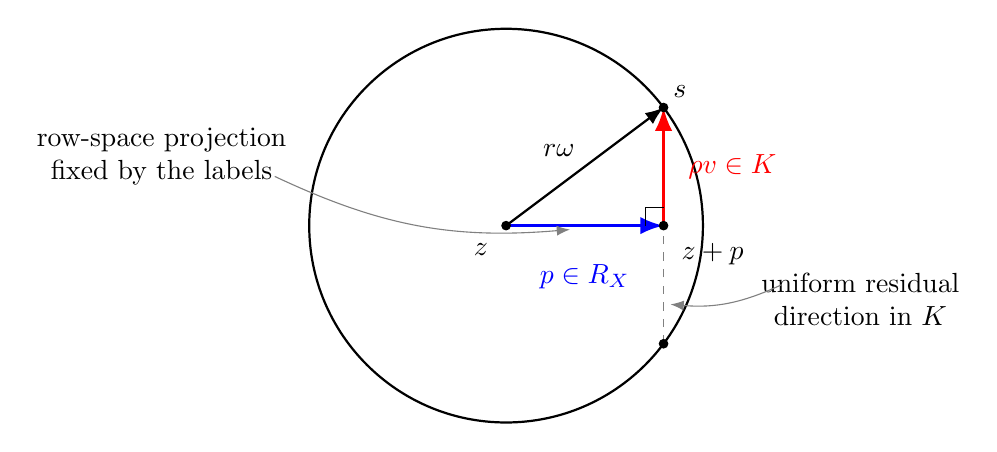
\begin{tikzpicture}[scale=1.25,>=Latex]
  \draw[thick] (0,0) circle (2);
  \draw[gray,dashed] (1.6,-1.2) -- (1.6,1.2);
  \draw[->,very thick,blue] (0,0) -- (1.6,0)
    node[midway,below=10pt] {\(p\in R_X\)};
  \draw[->,very thick,red] (1.6,0) -- (1.6,1.2)
    node[midway,right=5pt] {\(\rho v\in K\)};
  \draw[->,thick] (0,0) -- (1.6,1.2)
    node[midway,above left] {\(r\omega\)};
  \draw (1.42,0) -- (1.42,.18) -- (1.6,.18);
  \fill (0,0) circle (1.4pt) node[below left=3pt] {\(z\)};
  \fill (1.6,0) circle (1.4pt) node[below right=3pt] {\(z+p\)};
  \fill (1.6,1.2) circle (1.4pt) node[above right] {\(s\)};
  \fill (1.6,-1.2) circle (1.4pt);
  \node[align=center] at (-3.5,.7)
    {row-space projection\\fixed by the labels};
  \draw[->,gray] (-2.35,.5) to[bend right=15] (.65,-.04);
  \node[align=center] at (3.6,-.75)
    {uniform residual\\direction in \(K\)};
  \draw[->,gray] (2.8,-.6) to[bend left=15] (1.67,-.8);
\end{tikzpicture}

\caption{An orthogonal cross-section of the decomposition in
Lemma~\ref{s:residual}. The observed row-space component is
\(p=r\sqrt{1-t}\,e\); the remaining component has length
\(\rho=r\sqrt t\) and direction in \(K\).
The line meets the displayed circle in two points because this
cross-section is two-dimensional. In higher dimension the same
intersection is the residual subsphere \(z+p+\rho S(K)\).}
\label{s:residual-figure}
\end{figure}

Figure~\ref{s:residual-figure} shows the geometric content of the
conditioning. The subspaces in the lemma are analysis variables; the
learner is given exactly \(X,Xs\). The next consequence is the point
where the full data-dependent state choice is accounted for.

\begin{lemma}[Averaging after a block]\label{s:state-maximum}
In the setting of Lemma~\ref{s:residual}, let \(\mathcal V\) be nonempty and finite,
let \(g_v:S^{d-1}\to[0,1]\) be Borel, and let Borel weights
\(\kappa_v(X,y)\ge0\) satisfy \(\sum_v\kappa_v\le1\). Put
\[
 z'=z+r\sqrt{1-t}\,e,\qquad \rho=r\sqrt t,\qquad
 F_v(K)=\int g_v(z'+\rho u)\,d\sigma_K(u).
\]
Then
\begin{equation}\label{s:state-max-bound}
 \E_{X,s}\sum_v\kappa_v(X,Xs)g_v(s)
 \le \E_{t,e}\E_{K\mid e}\max_v F_v(K).
\end{equation}
The expectation on the left uses the independent uniform subsphere
target and Gaussian block.
\end{lemma}
\begin{proof}
Conditional on \(X,t,e\), the labels are \(Xz'\), the weights are
fixed, and \(u\) is uniform in \(K\). The conditional mean is
\(\sum_v\kappa_v(X,Xz')F_v(K)\), bounded by \(\max_vF_v(K)\).
This maximum no longer depends on the remaining matrix data except
through \(K\). The reversed-order part of Lemma~\ref{s:residual}
therefore gives the right side of \eqref{s:state-max-bound}.
\end{proof}

The maximum is taken before the matrix is replaced by its marginal
subspace law. It allows the selected state to depend arbitrarily on
the entire matrix and every exact label. No claim that a forward
posterior at a reached state is uniform on a subsphere is used.

\section{Caps and directions in a random subspace}\label{s:subspace-moments}

The residual law reduces a block to averages of continuation functions
on a random subspace. We first bound terminal success by spherical caps.
We then compute the dependence between several directions drawn in the
same random subspace. Both block methods will use this conditional law;
their different ways of bounding its moments come later.

\subsection{Caps and terminal outputs}

\begin{lemma}[Spherical caps]\label{s:caps}
Let \(e\) be a unit vector in a \(D\)-dimensional Euclidean space.
For \(D\ge3\) and every \(\delta>0\),
\begin{equation}\label{s:sharp-cap}
 \sigma_{\R^D}\{u:\norm{u-e}\le\delta\}
 \le \frac{c_D}{2}\delta^{D-1}
 \le \frac{\sqrt D}{2}\delta^{D-1}.
\end{equation}
For \(D\ge2\) and \(0\le\theta\le\pi\),
\begin{equation}\label{s:angular-cap}
 \sigma_{\R^D}\{u:\angle(u,e)\le\theta\}
 \le(2\theta)^{D-1}.
\end{equation}
Consequently, on an affine subsphere \(z+R S(H)\) as in
\eqref{s:affine-sphere}, with radius \(R\) and linear dimension
\(D\ge2\), the angular success probability of any
fixed unit output is at most
\begin{equation}\label{s:affine-terminal}
 \min\{1,(8\epsilon/R)^{D-1}\}.
\end{equation}
The last assertion also holds after averaging any target-independent
output law.
\end{lemma}
\begin{proof}
For the chordal cap, \(t=\ip ue\) lies in an interval of length at
most \(\delta^2/2\) next to \(1\), and \(1-t^2\le\delta^2\) on that
interval. Integrating \eqref{s:coordinate-density} with \(l=1\)
gives \eqref{s:sharp-cap}. For the angular cap, the polar-angle density
is proportional to \(\sin^{D-2}\phi\) on \([0,\pi]\). Its numerator
over \([0,\theta]\) is at most \(\theta^{D-1}/(D-1)\).
Its denominator is at least \(2^{-(D-2)}\), by integration over
\([\pi/6,5\pi/6]\). This proves \eqref{s:angular-cap}.

Angular error at most \(\epsilon\) between unit vectors implies
Euclidean error at most \(\epsilon\). After projection onto \(H\)
and division by \(R\), the successful directions in
\eqref{s:affine-sphere} lie in a Euclidean ball of radius
\(\epsilon/R\). If that set is nonempty, choose one successful
direction as a center. Every other successful direction has chordal
distance at most \(2\epsilon/R\) from it. For chordal distance
\(\delta\le2\), the corresponding angle is at most
\(2\arcsin(\delta/2)\le(\pi/2)\delta\). When \(8\epsilon/R<1\),
\eqref{s:angular-cap} therefore gives
\((8\epsilon/R)^{D-1}\); when \(8\epsilon/R\ge1\), total mass is
the asserted bound. Integrating this pointwise statement over an
independent output law proves the last claim.
\end{proof}

\subsection{Directions with a common random subspace}

The joint direction law below is a spherical form of the linear
Blaschke--Petkantschin formula; see Rubin
\cite[Corollary~3.2, equation~(3.5)]{Rubin2018}.
We derive the normalized conditional density directly.

\begin{lemma}[Conditional direction law]\label{s:directions}
Let \(E\) have dimension \(N\), let \(L\) be a uniform
\(K\)-dimensional subspace, and assume integers \(1\le h<K\le N\).
Conditional on \(L\), draw \(Y_1,\ldots,Y_h\) independently with
law \(\sigma_L\). Given \(Y_1,\ldots,Y_j\), their span \(V\) has
dimension \(j\) almost surely, and \(L\) is uniform among the
\(K\)-subspaces containing \(V\). For \(1\le j<h\), the conditional
density of \(Y_{j+1}\) relative to \(\sigma_E\) is
\begin{equation}\label{s:direction-density}
 \frac{c(K,j)}{c(N,j)}
 \dist(y,V)^{-(N-K)}
 \le \dist(y,V)^{-(N-K)}.
\end{equation}
For \(j=0\), the first marginal is \(\sigma_E\). If \(K=N\), the
density in \eqref{s:direction-density} is identically one.
\end{lemma}
\begin{proof}
Fix a \(K\)-space \(L_0\subset E\). Draw independent
\(\xi_1,\ldots,\xi_h\sim\sigma_{L_0}\) and an independent uniform
orthogonal matrix \(Q\), and put \(L=QL_0\), \(Y_i=Q\xi_i\).
This produces the stated experiment. Since \(h<K\), the first \(j\)
preimages, and hence their images, are linearly independent almost
surely.

Condition on the first \(j\) preimages and images. Applying
Gram--Schmidt to the preimages gives an orthonormal basis of their
span, and the images determine its image basis. Conditional on these
images, the action of \(Q\) on the perpendicular complement is a
uniform orthogonal isometry. It follows that
\[
 L=V\oplus L',\qquad
 L'\text{ uniform of dimension }K-j\text{ in }V^\perp.
\]
This conditional law depends only on \(V\), so it persists when the
preimages are forgotten.

The next preimage is still uniform in \(L_0\). Its projection onto
the preceding span has the \(j\)-coordinate density
\eqref{s:coordinate-density} in dimension \(K\). Its complementary
direction is sent by the uniform remaining isometry to a uniform
direction in \(V^\perp\), independently of that projection. The same
decomposition of a direction with law \(\sigma_E\) uses the coordinate
density in dimension \(N\). Taking their ratio gives
\[
 \frac{c(K,j)}{c(N,j)}
 (1-\norm{P_Vy}^2)^{-(N-K)/2},
\]
which is \eqref{s:direction-density}. The integral normalizing
\(c(K,j)\) is at least that normalizing \(c(N,j)\), because
\((1-\norm t^2)^{(K-j-2)/2}\ge
 (1-\norm t^2)^{(N-j-2)/2}\) on the unit ball. Thus the prefactor
is at most one. The first marginal is uniform by rotation invariance.
When \(K=N\), \(L=E\) and the original conditional draws remain
independent uniform directions, as the formula also shows.
\end{proof}


\section{Stopping and the remaining dimension budget}\label{s:stopping}

Each block estimate below loses two dimensions. Before iterating it,
we must know that enough dimensions remain. Terminal state counting
gives this fact on any putative short run. A separate full-data
argument covers constant accuracy. Both reductions count individual
samples and allow early stopping.

Throughout this section \(W=2^M\), and success is averaged over an
independent uniform signal. Logarithms denoted by \(\log_2\) are to
base two.

\begin{lemma}[Terminal count and padding]\label{s:terminal-count}
For \(d\ge3\), a learner of horizon \(T\) satisfies
\begin{align}
 \Prob(\mathrm{success})
 &\le (T+1)W(c_d/2)\epsilon^{d-1},\label{s:output-count-sharp}\\
 \Prob(\mathrm{success})
 &\le (T+1)W(2\epsilon)^{d-1}.\label{s:output-count-angular}
\end{align}
The learner can be padded to any prescribed later sample layer, with
the same success law and width at most
\begin{equation}\label{s:padded-width}
 W_*=(T+2)W.
\end{equation}
\end{lemma}
\begin{proof}
Fix a seed realization covered by Lemma~\ref{s:borel} and use its
Borel version. Its initial-state law is independent of the signal.
For each terminal index-state pair \((t,v)\), let \(q_{t,v}(s)\)
be its probability of being reached at signal \(s\), and let
\(\pi_{t,v}\) be its target-independent output law. There are at most
\((T+1)W\) such pairs. Replacing \(q_{t,v}(s)\) by one, then integrating
\(\pi_{t,v}\) over the uniform signal, bounds that pair's contribution
by a single angular cap mass. Angular success implies chordal error
at most \(\epsilon\), so \eqref{s:sharp-cap} gives
\eqref{s:output-count-sharp}; \eqref{s:angular-cap} gives
\eqref{s:output-count-angular}. The same numerical
bound holds for almost every fixed seed, so Lemma~\ref{s:borel}
permits averaging the original conditional success probabilities.

To pad, keep every halted state together with its original stopping
index as an absorbing state, and ignore later samples. At the final
layer use its original output law. At any layer there are at most
\(W\) active states and \((T+1)W\) halted index-state labels,
giving \eqref{s:padded-width}. This includes a stop at index zero.
\end{proof}

The terminal count also identifies the regime where the output
restriction alone is decisive. At success probability at least
\(2/3\), \eqref{s:output-count-sharp} gives
\[
 T+1\ge \frac{4}{3c_d}\,2^{-M}\epsilon^{-(d-1)}.
\]
For a fixed \(\alpha>0\), accuracy \(\epsilon=2^{-\alpha d}\)
therefore requires \(T\ge2^{(\alpha-o(1))d^2}\) when
\(M=o(d^2)\). The block arguments provide an additional obstruction beyond terminal
output counting. To apply them, we next extract the
remaining dimension budget from the same terminal count.

\begin{lemma}[Short-run dimension budget]\label{s:short-run}
Fix constants \(c>0\) and \(\alpha>0\), and put
\(L=\log_2(1/\epsilon)\). Suppose \(M(d)=o(d^2)\). On any sequence
of dimensions where uniform-prior success is at least \(\alpha\)
and \(T\le cdL\), one has
\begin{equation}\label{s:short-run-conclusions}
 L=o(d),\qquad T=o(d^2),\qquad \log_2 W_*=o(d^2).
\end{equation}
Consequently, for any block length \(k\ge c_0d\) with fixed \(c_0>0\),
\(\lceil T/k\rceil=o(d)\) on that sequence.
\end{lemma}
\begin{proof}
Since \(L\ge1\), \(T+1\le(c+1)dL\) and
\(\log_2 L\le L\). Taking logarithms in
\eqref{s:output-count-sharp} and using \(c_d\le\sqrt d\) gives the
estimate
\begin{equation}\label{s:sharp-short-run}
 (d-2)L
 \le M+\frac32\log_2d+\log_2\frac{c+1}{2\alpha}.
\end{equation}
This proves \(L=o(d)\), uniformly in the accuracy and the rules on
the indicated dimensions. The assumed sample bound gives
\(T=o(d^2)\); then \(\log_2 W_*=M+\log_2(T+2)=o(d^2)\).
Dividing \(T\) by \(k\ge c_0d\) proves the block-count assertion.

The short-run hypothesis is essential: the conclusion
\(L=o(d)\) applies only on the indicated dimensions.
\end{proof}

\begin{lemma}[Full-data residual bound]\label{s:full-data}
Let \(0\le T\le d-3\). Give an estimator all \(T\) Gaussian rows and
labels for a uniform signal, and allow any unit output depending on
these data and independent randomness. Put \(D=d-T\). For every
\(0<r_0<1\), its angular success probability is at most
\begin{equation}\label{s:full-data-bound}
 \frac{T}{d(1-r_0^2)}
 +\min\left\{1,\ \frac{c_D}{2}(2\epsilon/r_0)^{D-1},\
                    (8\epsilon/r_0)^{D-1}\right\}.
\end{equation}
\end{lemma}
\begin{proof}
For \(T\ge1\), the row span \(R_X\) has dimension \(T\) almost surely.
Given the full rows and labels, the row-space projection \(p=P_{R_X}S\)
is known, because the row matrix is injective on its row span.
The residual law is
\[
 S=p+rU,\qquad r=\sqrt{1-\norm p^2},\qquad
 U\sim\sigma_{R_X^\perp}.
\]
Conditional on the data, the residual direction is uniform.
At a fixed row span, spherical symmetry gives
\(\E\norm p^2=T/d\). Markov's inequality yields
\(\Prob(r<r_0)\le T/[d(1-r_0^2)]\).
On \(r\ge r_0\), successful residual directions lie in a chordal
cap of radius \(2\epsilon/r_0\), by the recentering argument in
Lemma~\ref{s:caps}. The sharp and affine terminal cap bounds give the
three alternatives in the minimum. The output randomization may be
averaged after conditioning on the full data. When \(T=0\), take
\(R_X=\{0\}\), \(p=0\), and \(r=1\); the same argument uses the
original full sphere.
\end{proof}

For \(T\le d/4\), take \(r_0=1/2\) in
\eqref{s:full-data-bound}. Since \(D\ge3d/4\) and
\(2\epsilon/r_0\le0.4\),
\[
 \Prob(\mathrm{success})
 \le\frac13+(c_D/2)0.4^{D-1}=\frac13+o(1)
\]
uniformly in this range of \(T\). Thus uniform-prior success at least
\(1/2\) requires
\begin{equation}\label{s:quarter-endpoint}
 T>d/4
\end{equation}
for all sufficiently large \(d\).



These full-data estimates apply to a learner that stopped earlier,
because revealing all pre-generated rows and labels only gives it
more information.

\section{A beta-mixture comparison and the explicit constant}\label{s:beta-mixture}

A block leaves a uniform direction in a random residual subspace. To
bound a high moment of its continuation average, we must control the
next direction after earlier directions in that same subspace have
been exposed. Lemma~\ref{s:directions} describes this law; the next
lemma compares it with two families of tests on which an affine
suffix bound can be used directly.

The first test is the whole ambient sphere. The second fixes one
direction from the span of the earlier draws and averages on a
latitude perpendicular to that direction. If the ambient space has
linear dimension \(D'\), each such latitude has linear dimension
\(D'-1\), regardless of the number of earlier draws. This is the
reason that a block will spend only two test dimensions: one for the
observed projection direction and one for the comparison latitude.
The beta variable in the construction below chooses the latitude
radius so that its law controls the next direction near the preceding
span.

\begin{lemma}[Two-component domination]\label{s:mixture}
Let \(E\) have dimension \(D'\), let \(V\subset E\) have dimension
\(1\le j<n<D'\), and let \(N\) be uniform among the \(n\)-dimensional
subspaces containing \(V\). Conditional on \(N\), let \(v\) be
uniform on \(S(N)\). Set
\[
 \alpha=\frac{n-j}{2},\qquad
 \alpha_*=\frac{D'-j}{2},\qquad
 \beta_0=\frac j2,\qquad
 \beta_1=\frac{D'-n+j-1}{2}.
\]
Let \(\nu_0=\sigma_E\). Let \(\nu_1\) be the law of
\begin{equation}\label{s:mixture-construction}
 \sqrt{1-Z}\,e_0+\sqrt Z\,u_0,\qquad
 Z\sim\Beta(\alpha,\alpha_*-\alpha),\quad
 e_0\sim\sigma_V,\quad
 u_0\mid e_0\sim\sigma_{E\cap e_0^\perp},
\end{equation}
where \(Z\) is independent of the directions. Then, as positive
measures on \(S(E)\),
\begin{equation}\label{s:mixture-domination}
 \Law(v)\le2^{D'}(\nu_0+\nu_1).
\end{equation}
For \(j=0\), the first direction averaged over a uniform \(N\) is
uniform on \(S(E)\). If \(n=D'\), then \(N=E\) and each new
independent direction is uniform even after earlier directions are
conditioned on. These cases require no mixture.
\end{lemma}
\begin{proof}
Put \(Q(y)=\norm{P_{V^\perp}y}^2\). For the actual direction, the
orthogonal decomposition \(N=V\oplus(N\cap V^\perp)\) and
Lemma~\ref{s:coordinates} give
\[
 Q(v)\sim\Beta(\alpha,\beta_0).
\]
For \(\nu_0\), the fraction has law
\(\Beta(\alpha_*,\beta_0)\). Under \(\nu_1\), it equals \(ZX\),
where \(X=\norm{P_{V^\perp}u_0}^2\). If \(j>1\), the decomposition
\[
 E\cap e_0^\perp=V^\perp\oplus(V\cap e_0^\perp)
\]
gives \(X\sim\Beta(\alpha_*,(j-1)/2)\), independently of \(Z\).
The beta-product identity \eqref{s:beta-product} gives
\(Q\sim\Beta(\alpha,\beta_1)\). If \(j=1\), the second summand is
zero and \(X=1\) deterministically. In that case
\(\beta_1=\alpha_*-\alpha\), so \(Q=Z\) has the same stated law.
We do not use a beta law with second shape zero.

The three vector laws are invariant under independent orthogonal
transformations of \(V\) and \(V^\perp\). Their two component lengths
are nonzero almost surely. For completeness, average a bounded Borel
function of a vector over an independent uniform element of
\(O(V)\times O(V^\perp)\). At fixed nonzero component lengths, this
average is integration over the product of the two uniform direction
laws. Invariance leaves the original expectation unchanged, including
after multiplication by any bounded function of \(Q\). Thus each
vector law is obtained from its scalar \(Q\) law with the same
independent uniform component directions. A comparison of the scalar
densities therefore lifts to the full vector measures.

Write \(b=D'+1-n\). The nontrivial case has \(b\ge2\), and
\[
 \alpha_*-\alpha=(b-1)/2>0,\qquad
 \beta_1-\beta_0=(b-2)/2\ge0.
\]
Let \(f_{A,B}\) denote the normalized beta density. The beta integral
decreases when either positive shape parameter increases. For
\(q\ge1/2\),
\[
 \frac{f_{\alpha,\beta_0}(q)}{f_{\alpha_*,\beta_0}(q)}
 =\frac{\mathrm B(\alpha_*,\beta_0)}
        {\mathrm B(\alpha,\beta_0)}
       q^{-(\alpha_*-\alpha)}
 \le2^{\alpha_*-\alpha}\le2^{D'}.
\]
For \(q<1/2\),
\[
 \frac{f_{\alpha,\beta_0}(q)}{f_{\alpha,\beta_1}(q)}
 =\frac{\mathrm B(\alpha,\beta_1)}
        {\mathrm B(\alpha,\beta_0)}
       (1-q)^{-(\beta_1-\beta_0)}
 \le2^{\beta_1-\beta_0}\le2^{D'}.
\]
This includes equality \(\beta_1=\beta_0\) when \(b=2\).
Splitting at \(1/2\) and using the common direction factors proves
\eqref{s:mixture-domination}. For \(j=0\), rotation invariance gives
the uniform marginal; for \(n=D'\), the subspace is the whole \(E\)
and the original draws remain independent uniform directions.
\end{proof}

\begin{proof}[Proof of Theorem~\ref{s:main}]
Fix the memory sequence, and suppose that the conclusion fails along
an unbounded sequence of dimensions. All logarithms in this proof
are to base two. Write
\begin{equation}\label{s:numeric-contradiction}
 \lambda=\log_2(1/\epsilon),\qquad
 c_*=2^{-16},\qquad T<c_*d\lambda.
\end{equation}

\paragraph{The short-run reduction.}
Lemma~\ref{s:short-run}, with \(c=c_*\) and \(\alpha=2/3\), gives
\(\lambda=o(d)\), \(T=o(d^2)\), and
\(\log_2w=o(d^2)\) for the padded width
\[
 w=(T+2)2^M.
\]
These bounds are uniform over the violating accuracies and learner
rules: the explicit estimate \eqref{s:sharp-short-run} bounds
\((d-2)\lambda\) by a function of \(d\) and \(M(d)\) alone.
If \(\lambda\le1024\), then \(T<d/64\), contradicting the
full-data bound \eqref{s:quarter-endpoint} at large \(d\).
We therefore restrict to \(\lambda>1024\).

Set
\begin{equation}\label{s:numeric-parameters}
 k=m=\lfloor d/16\rfloor,\qquad
 p=2\lfloor d/32\rfloor,\qquad
 \ell=p/2,\qquad
 J=\lceil T/k\rceil,\qquad
 G=2^{4d}w^{1/m}.
\end{equation}
The radius exponent \(p\) is even, so the inverse-radius moments
below have the integer exponent \(\ell=p/2\).
Pad early stops to length \(T\) using
Lemma~\ref{s:terminal-count}, and divide the horizon into \(J\)
batches of length at most \(k\). A short last batch retains its actual
positive length. When \(T=0\), there are no batches. At sufficiently
large violating dimensions,
\begin{equation}\label{s:numeric-budget}
 J\le32c_*\lambda+1=o(d),\qquad
 J\le d/8,\qquad m,p\ge d/32.
\end{equation}
The first inequality uses \(k\ge d/32\).

\paragraph{The suffix bound.}
Fix a rule seed for which Lemma~\ref{s:borel} applies, and use its
Borel version. The signal remains uniform and independent of the
pre-generated rows and initialization. Start a continuation from any
specified boundary state, without conditioning on whether that state
is reached. All the bounds below are uniform over this fixed choice
of rules and state.

For a boundary state \(v\) after \(i\) batches, let \(h_{i,v}(s)\)
be its Borel suffix success. We claim that every affine subsphere
\(c+rS(H)\) with \(D=\dim H\ge d-2i\) satisfies
\begin{equation}\label{s:numeric-invariant}
 \int h_{i,v}(c+ru)\,d\sigma_H(u)
 \le G^{J-i}(8\epsilon/r)^p.
\end{equation}
The test dimension in this assertion decreases by two as the
boundary index increases. In the backward step from \(i+1\) to
\(i\), the available bounds therefore include all affine tests of
dimensions \(D-1\) and \(D-2\), whenever the current test has
dimension \(D\ge d-2i\).

At \(i=J\), Lemma~\ref{s:caps} proves the claim. Indeed
\(D\ge d-2J\ge3d/4\) gives \(D-1\ge p\); if
\(8\epsilon/r\ge1\), use total mass, and otherwise compare the
exponents in \eqref{s:affine-terminal}. This also treats \(J=0\).

\paragraph{One block.}
Suppose the claim holds at \(i+1\), and let the next batch have length
\(1\le b\le k\). Lemma~\ref{s:residual} gives
\[
 \rho^2\sim\Beta((D-b)/2,b/2),\qquad
 c'=c+r\sqrt{1-\rho^2}\,e,\qquad r'=r\rho,
\]
\[
 E=H\cap e^\perp,\qquad D'=D-1,\qquad n=D-b.
\]
Conditional on \(\rho,e\), the residual space \(N\) is uniform of
dimension \(n\) in \(E\). By Lemma~\ref{s:state-maximum}, the
left side of \eqref{s:numeric-invariant} is at most
\begin{equation}\label{s:numeric-max}
 \E_{\rho,e}\E_N\max_{v'}F_{v'}(N),\qquad
 F_{v'}(N)=\int h_{i+1,v'}(c'+r'u)\,d\sigma_N(u).
\end{equation}
This step keeps all dependence on the exact batch data until the state
maximum has been taken.

We bound this state maximum through an \(m\)-th moment. Each
conditional factor in that moment will use the same stage-\(i+1\)
affine bound; the earlier replica span changes its distribution but
not the induction stage.

Fix \(\rho,e,v'\) and write
\[
 U_0=G^{J-i-1}(8\epsilon/r')^p.
\]
Expand \(F_{v'}(N)^m\) using \(m\) directions drawn independently
conditional on \(N\). Given the first \(j<m\) directions, their
span \(V\) has dimension \(j\) almost surely, and
Lemma~\ref{s:directions} makes \(N\) uniform among the \(n\)-spaces
containing \(V\). The parameter bounds imply
\[
 D\ge3d/4,\qquad n\ge11d/16,\qquad m\le d/16<n.
\]
For \(j=0\), the next direction is uniform on \(S(E)\), and
the stage \(i+1\) hypothesis bounds its expected success factor by
\(U_0\), since \(D'=D-1\ge d-2(i+1)\). If \(b=1\), then
\(n=D'\) and every next independent direction is uniform in \(E\);
the same bound applies. These cases precede any use of a beta mixture.

For \(j\ge1\) and \(b\ge2\), apply Lemma~\ref{s:mixture}. The
\(\nu_0\) expectation is at most \(U_0\). Under \(\nu_1\),
conditional on \(Z,e_0\), the target is uniform on the affine
subsphere with
\[
 \widetilde H=E\cap e_0^\perp,\qquad
 \widetilde c=c'+r'\sqrt{1-Z}\,e_0,\qquad
 \widetilde r=r'\sqrt Z.
\]
Its linear dimension is \(D-2\ge d-2(i+1)\). Also
\(\widetilde c\perp\widetilde H\), \(\widetilde r>0\), and
\(\norm{\widetilde c}^2+\widetilde r^2=1\), because \(c'\perp E\)
and \(\norm{c'}^2+(r')^2=1\). The induction hypothesis bounds its
mean by \(U_0Z^{-\ell}\).

In the notation of Lemma~\ref{s:mixture},
\[
 n-j\ge10d/16,\qquad
 \alpha-\ell\ge9d/32\ge d/4,\qquad
 \alpha_*\le d/2.
\]
The other shape \(\alpha_*-\alpha=(b-1)/2\) is positive.
The integer \(\ell=\lfloor d/32\rfloor\) is strictly below the
first shape, and every ratio below is at most two:
\begin{equation}\label{s:mixture-inverse}
 \E Z^{-\ell}
 =\prod_{t=1}^{\ell}\frac{\alpha_*-t}{\alpha-t}
 \le2^\ell\le2^d.
\end{equation}
Since \(D'\le d\), the mixture domination bounds the conditional
expected next factor by
\[
 2^dU_0(1+\E Z^{-\ell})\le2^{3d}U_0.
\]
For each preceding replica span, this uses a fresh test in the same
dimension \(D-2\). Only the single direction \(e_0\) is removed from
\(E\); no dimension decrease is carried from one replica to the next.

Integrating the nonnegative product in reverse conditional order gives
\[
 \E_NF_{v'}(N)^m\le(2^{3d}U_0)^m.
\]
Jensen's inequality and the sum of the at most \(w\) state moments
then give
\[
 \E_N\max_{v'}F_{v'}(N)\le w^{1/m}2^{3d}U_0.
\]
For the residual fraction \(\rho^2\), the first shape satisfies
\(n/2-\ell\ge5d/16\ge d/4\), its total shape is \(D/2\le d/2\),
and its other shape \(b/2\) is positive even for a one-row batch.
The same integer beta identity yields
\begin{equation}\label{s:residual-inverse-numeric}
 \E\rho^{-p}
 =\prod_{t=1}^{\ell}\frac{D/2-t}{n/2-t}
 \le2^\ell\le2^d.
\end{equation}
Averaging \(r'=r\rho\) in \eqref{s:numeric-max} supplies the factor
\(w^{1/m}2^{4d}=G\), completing the backward induction.

\paragraph{The numerical conclusion.}
At \(i=0\), take the full sphere \(H=\R^d,c=0,r=1\).
The bound is uniform in the fixed shared seed and initial state;
joint independence permits averaging over initialization, and then
Lemma~\ref{s:borel} permits averaging the original measurable
conditional success probabilities over the seed. By
\(\log_2w=o(d^2)\) and \(m\ge d/32\), we have
\(\log_2G\le5d\) eventually. The base-two logarithm of the success
upper bound is at most
\begin{align}
 5d(32c_*\lambda+1)+p(3-\lambda)
 &\le5d+(160c_*-1/64)d\lambda\notag\\
 &\le5d-d\lambda/128\le-3d.\label{s:numeric-arithmetic}
\end{align}
Here \(3-\lambda\le-\lambda/2\), \(p\ge d/32\),
\(160c_*=5/2048\le1/128\), and \(\lambda\ge1024\).
The resulting success is less than \(2/3\), a contradiction.

Both precision branches exclude an unbounded sequence of violations.
All eventual conditions were bounded using
\eqref{s:sharp-short-run} and the fixed memory sequence; the
full-data cap threshold is absolute. This proves the uniform
dimension threshold and \eqref{s:main-bound}.
\end{proof}

\section{The radius-weighted block estimate}\label{s:weighted-proof}

We now develop the cap-moment method for arbitrary bounded continuation
functions. Weighting the mean on an affine subsphere by a power of its
radius makes the same test useful at every scale. The resulting block
inequality is independent of a learner and also gives a precision bound
at success probability one half.

For a Borel function \(g:S^{d-1}\to[0,1]\), an exponent \(a=d/16\), and an integer
\(1\le n\le d\), define
\begin{equation}\label{s:weighted-norm}
 B_n(g)=\sup_{\substack{\dim H=n\\ z\perp H,\ R>0\\
                         \norm z^2+R^2=1}}
 R^a\int g(z+R\omega)\,d\sigma_H(\omega).
\end{equation}
In particular \(B_d(g)=\int g\,d\sigma_{\R^d}\). The radius weight
allows small subspheres to carry more mass while keeping the same test
at every scale.

The block may choose among arbitrary bounded continuation functions.

\begin{theorem}[Radius-weighted block estimate]\label{s:weighted-theorem}
There are absolute constants \(C\ge1\) and \(d_*\) such that the
following holds for every integer \(d\ge d_*\). Put
\[
 k=m=\lfloor d/16\rfloor,\qquad a=d/16.
\]
Let \(W\ge1\), let \(\mathcal V\) be a nonempty finite set with
\(|\mathcal V|\le W\), and let
\(\kappa_v:\R^{k\times d}\times\R^k\to[0,1]\) be Borel functions
with \(\sum_{v\in\mathcal V}\kappa_v\le1\). For Borel
\(g_v:S^{d-1}\to[0,1]\), set
\[
 g_{\rm in}(s)=
 \E_X\sum_{v\in\mathcal V}\kappa_v(X,Xs)g_v(s),
\]
where \(X\) has \(k\) independent \(N(0,I_d)\) rows. For every integer
\(n\) with \(d/2\le n\le d\),
\begin{equation}\label{s:weighted-block}
 B_n(g_{\rm in})
 \le W^{1/m}C^d\max_{v\in\mathcal V}B_{n-2}(g_v).
\end{equation}
If \(\epsilon>0\), \(\pi\) is any probability measure on \(S^{d-1}\) and
\[
 g_\pi(s)=\int\ind_{\{\arccos\ip us\le\epsilon\}}\,\pi(du),
\]
then, in the same range of \(n\),
\begin{equation}\label{s:weighted-terminal}
 B_n(g_\pi)\le C^d\epsilon^a.
\end{equation}
\end{theorem}

The width factor pays for selecting a continuation after the block.
The two-dimensional change instead records the latitude tests used to
bound each conditional direction average. We first establish the moment
estimate that connects these two features.

\subsection{Caps and subspace moments}

The use of replica moments and successive orthogonalization is related
to Sharan, Sidford, and Valiant \cite[Section~7, Lemma~12]{SSV2019}.
The density becomes large near the preceding span. The next lemma
shows that a cap estimate with sufficient dimension slack makes this
singularity integrable. Its explicit constant retains a useful
quantitative form of the argument.

\begin{lemma}[Caps and subspace moments]\label{s:cap-moment}
Let \(E\) have dimension \(N\le d\), and let \(L\) be a uniform
\(K\)-space in \(E\), with integers \(1\le h<K\le N\). Put
\(b=N-K\). Let \(f:S(E)\to[0,1]\) be Borel. Suppose that for some
finite \(\Lambda\ge0\), constants \(A_0,A_1\ge1\), and
\(0\le a<N-1\),
\begin{align}
 \int f\,d\sigma_E&\le A_0^d\Lambda,\label{s:cap-total}\\
 \int_{\norm{y-y_0}\le\delta}f(y)\,d\sigma_E(y)
 &\le A_1^d\Lambda\delta^{N-1-a}
 \quad(y_0\in S(E),\ \delta>0).\label{s:cap-hypothesis}
\end{align}
If
\begin{equation}\label{s:moment-margin}
 N-1-a-(h-1)-b\ge1,
\end{equation}
then
\begin{equation}\label{s:moment-bound}
 \E_L\left(\int f\,d\sigma_L\right)^h
 \le\left([4\max\{A_0,9A_1\}]^d\Lambda\right)^h.
\end{equation}
For a nonempty family of at most \(W\) functions satisfying the same
conditions with numbers \(\Lambda_v\),
\begin{equation}\label{s:moment-maximum}
 \E_L\max_v\int f_v\,d\sigma_L
 \le W^{1/h}[4\max\{A_0,9A_1\}]^d\max_v\Lambda_v.
\end{equation}
In particular, \(A_0=1,A_1=4\) gives the constant \(144^d\).
\end{lemma}
\begin{proof}
Put \(\alpha=N-1-a\) and \(Q_0=\max\{A_0,9A_1\}\).
For a \(j\)-dimensional subspace \(V\subset E\), \(1\le j<h\),
and \(0<\delta<1\), every sphere point within distance \(\delta\)
of \(V\) lies within \(2\delta\) of its normalized projection onto
\(S(V)\). A maximal \(\delta\)-separated subset of \(S(V)\) has at
most \((3/\delta)^j\) points: the open balls of radius \(\delta/2\)
about them are disjoint inside the ball of radius \(1+\delta/2\)
in \(V\). Caps of radius \(3\delta\) about these points cover the
tube. Hence
\begin{equation}\label{s:tube}
 \int_{\dist(y,V)\le\delta}f\,d\sigma_E
 \le A_1^d3^{\alpha+j}\Lambda\delta^{\alpha-j}
 \le Q_0^d\Lambda\delta^{\alpha-j}.
\end{equation}
The last inequality uses \(\alpha,j\le d\). At \(\delta=1\), the
same bound follows from \eqref{s:cap-total}. The zero-distance set
has sphere measure zero because \(j<N\). The shells
\(2^{-i-1}<\dist(y,V)\le2^{-i}\) therefore give
\begin{align}
 \int f(y)\dist(y,V)^{-b}\,d\sigma_E(y)
 &\le Q_0^d\Lambda\,2^b
       \sum_{i\ge0}2^{-i(\alpha-j-b)}\notag\\
 &\le Q_0^d\Lambda\,2^{b+1}
 \le (4Q_0)^d\Lambda.\label{s:inverse-distance}
\end{align}
Here \(\alpha-j-b\ge1\) follows from
\eqref{s:moment-margin}, and \(b+1\le2d\). For \(j=0\), the distance
of a unit vector from \(\{0\}\) is one and the same conclusion follows
directly from total mass. Thus this case needs neither a net nor a
shell sum.

Conditional on \(L\), draw \(Y_1,\ldots,Y_h\) independently from
\(\sigma_L\). Expanding the power in \eqref{s:moment-bound} gives
\(\E\prod_{i=1}^h f(Y_i)\).
Lemma~\ref{s:directions} and \eqref{s:inverse-distance} bound the last
conditional factor by \((4Q_0)^d\Lambda\). Continue in reverse
conditional order, using total mass for the first direction. This
proves \eqref{s:moment-bound}. Finally, writing
\(F_v(L)=\int f_v\,d\sigma_L\), Jensen's inequality gives
\[
 \E\max_vF_v(L)
 \le\E\left(\sum_vF_v(L)^h\right)^{1/h}
 \le\left(\sum_v\E F_v(L)^h\right)^{1/h},
\]
which proves \eqref{s:moment-maximum}.
\end{proof}

The lemma pays for the span of prior replicas through the tube
exponent. It does not spend a new induction dimension for each
replica: every conditional factor is tested against the same cap
hypothesis on \(S(E)\). In the applications, one latitude of an
affine subsphere supplies that hypothesis.

\subsection{Proof of the block estimate and its application}

A latitude in the perpendicular ambient sphere has two fewer linear
dimensions than the original test. Its radius-weighted mean supplies the cap hypothesis;
a final beta integral averages the residual radius.

\begin{proof}[Proof of Theorem~\ref{s:weighted-theorem}]
We work at sufficiently large \(d\), with the parameters in the
theorem. First consider a terminal function \(g_\pi\) and a test
\((z,H,R)\) of dimension \(n\ge d/2\). If \(R\ge2\epsilon\), the
successful directions for any fixed output lie in a chordal cap of
radius \(2\epsilon/R\le1\). By \eqref{s:sharp-cap}, their mass is at
most \((c_n/2)(2\epsilon/R)^{n-1}\). Since \(n-1\ge a\),
multiplication by \(R^a\) bounds this by
\((c_n/2)(2\epsilon)^a\le C^d\epsilon^a\).
If \(R<2\epsilon\), total mass gives \(R^a\le(2\epsilon)^a\).
Averaging the output law proves \eqref{s:weighted-terminal}.

For the block bound, fix a test \((z,H,R)\) of dimension \(n\).
Let \(V\) be the span in \(H\) of the \(k\) projected rows. Put
\[
 p=R P_V\omega,\qquad r=\sqrt{R^2-\norm p^2},\qquad
 K=H\cap V^\perp,\qquad q=n-k.
\]
Almost surely \(p\ne0\) and \(r>0\). Conditional on the matrix and
\(p\), the target is \(z+p+rU\) with \(U\sim\sigma_K\), and its
labels are \(X(z+p)\). Lemma~\ref{s:state-maximum} bounds the
averaged block function by
\begin{equation}\label{s:weighted-max}
 \E_p\E_{K\mid p}\max_v
       \int g_v(z+p+rU)\,d\sigma_K(U).
\end{equation}
Here \(K\mid p\) is uniform among the \(q\)-spaces of
\(H'=H\cap p^\perp\), whose dimension is \(N=n-1\).
Indeed, the length of \(p\) fixes the beta fraction, its direction
fixes \(e\), and Lemma~\ref{s:residual} gives this conditional law.

Fix \(p\) and one function \(g=g_v\). On \(S(H')\) set
\[
 f(U)=g(z+p+rU),\qquad \Lambda=r^{-a}B_{n-2}(g).
\]
For \(w\in S(H')\), condition on the latitude coordinate
\(t=\ip Uw\in(-1,1)\). The target on that latitude is uniform on
\[
 z+p+rtw+r\sqrt{1-t^2}\,S(H'\cap w^\perp).
\]
This is an admissible affine subsphere of linear dimension \(n-2\):
its center is perpendicular to \(H'\cap w^\perp\), and its squared
center norm plus squared radius is
\(\norm z^2+\norm p^2+r^2=1\). The definition of \(B_{n-2}\) therefore
bounds the latitude average of \(f\) by
\(\Lambda(1-t^2)^{-a/2}\).

The coordinate density in dimension \(N\) has remaining exponent
\((N-3-a)/2\ge0\). Integrating it over the whole interval and then
over the cap interval gives
\begin{align}
 \int f\,d\sigma_{H'}&\le2c_N\Lambda,\label{s:weighted-total}\\
 \int_{\norm{U-w}\le\eta} f(U)\,d\sigma_{H'}(U)
 &\le c_N\Lambda\eta^{N-1-a}
 \qquad(0<\eta\le1).\label{s:weighted-cap}
\end{align}
For the second line the coordinate interval has length at most
\(\eta^2/2\) and \(1-t^2\le\eta^2\) there. For \(\eta>1\), total
mass extends the cap bound with an absolute exponential factor.
Since \(2c_N\le2\sqrt d\le4^d\), these estimates satisfy
Lemma~\ref{s:cap-moment} with absolute \(A_0,A_1\).

Use that lemma with ambient dimension \(N=n-1\), subspace dimension
\(q=n-k\), and moment \(m=k\). The singular power is
\(N-q=k-1\). The required inequalities hold at large \(d\):
\(1\le m<q\le N\), \(0\le a<N-1\), and, for
\(0\le l<m\),
\[
 N-1-a-l-(N-q)
 =n-1-a-l-k
 \ge n-a-2k
 \ge5d/16\ge1.
\]
The moment conclusion is
\begin{equation}\label{s:weighted-moment}
 \E_{K\mid p}\left(\int g(z+p+rU)\,d\sigma_K(U)\right)^m
 \le\left(C^d r^{-a}B_{n-2}(g)\right)^m.
\end{equation}
Each replica uses the same \(n-2\)-dimensional latitude tests.
No additional induction dimension is lost while the replicas are
integrated.

The maximum inequality \eqref{s:moment-maximum} now bounds the inner
expectation in \eqref{s:weighted-max} by
\[
 W^{1/m}C^d r^{-a}\max_v B_{n-2}(g_v).
\]
It remains to average the residual radius. By
Lemma~\ref{s:residual}, \(t=(r/R)^2\sim\Beta(q/2,k/2)\).
The denominator of its beta integral satisfies
\[
 \mathrm B(q/2,k/2)
 \ge \frac12\,4^{-(q/2-1)_+-(k/2-1)_+}
 \ge 4^{-d},
\]
by restriction to \([1/4,3/4]\), where \(x_+=\max\{x,0\}\).
After multiplication by \(t^{-a/2}\), the numerator is
\begin{equation}\label{s:weighted-beta-integral}
 \int_0^1 t^{(q-a)/2-1}(1-t)^{k/2-1}\,dt\le2.
\end{equation}
Indeed \(q-a\ge2\) makes the first exponent nonnegative. If \(k\ge2\)
the second is also nonnegative; if \(k=1\), its integral is at most
\(\int_0^1(1-t)^{-1/2}\,dt=2\). Thus
\(\E(R/r)^a\le C^d\). This direct beta-integral argument does not
require \(a/2\) to be an integer. Multiplying
\eqref{s:weighted-max} by \(R^a\), averaging, and taking the supremum
over the original test proves \eqref{s:weighted-block}.
\end{proof}

The block theorem now gives a complete lower bound from these norms.
This application uses success \(1/2\), which is enough for the
constant-accuracy estimate \eqref{s:quarter-endpoint}.

\begin{corollary}[Precision bound from radius weights]\label{s:weighted-application}
There is an absolute \(c>0\) such that, for every \(M(d)=o(d^2)\),
all sufficiently large \(d\), and all \(0<\epsilon\le1/10\), a learner
with uniform-prior angular success at least \(1/2\) satisfies
\[
 T\ge c\,d\log_2(1/\epsilon).
\]
The eventual threshold may depend on the memory sequence.
\end{corollary}
\begin{proof}
Put \(L=\log_2(1/\epsilon)\). The dimensions with \(T\ge dL\)
already satisfy the conclusion. On the remaining dimensions,
Lemma~\ref{s:short-run}, using
\eqref{s:sharp-short-run}, gives \(L=o(d)\), \(T=o(d^2)\), and
\(\log_2 W_*=o(d^2)\). Pad to \(b=\lceil T/k\rceil=o(d)\) blocks
of \(k=\lfloor d/16\rfloor\) samples with width \(W_*\), as in
Lemma~\ref{s:terminal-count}. A short final block is filled with
unused fresh rows.

Let \(G_{i,v}\) be the Borel suffix success from state \(v\) after
\(i\) blocks. Recursion \eqref{s:recursion} and
Theorem~\ref{s:weighted-theorem} apply at each boundary. Use dimension
\(n=d-2i\) at stage \(i\). For all sufficiently large dimensions
under consideration, every needed dimension, including the terminal
one, satisfies
\begin{equation}\label{s:weighted-budget}
 d-2i\ge d-2b\ge d/2\qquad(0\le i\le b).
\end{equation}
Iteration of \eqref{s:weighted-block}, followed by
\eqref{s:weighted-terminal}, gives
\begin{equation}\label{s:weighted-iteration}
 \frac12\le
       [W_*^{1/m}C^d]^b C^d\epsilon^a.
\end{equation}
The same bound holds for each initial state and each fixed independent
choice of rules, so averaging them is legitimate.

At large \(d\), \(m\ge d/32\) and
\(\log_2 W_*/m\le d\). Taking base-two logarithms in
\eqref{s:weighted-iteration}, with \(a=d/16\), gives
\(L\le C_1(b+1)\) for an absolute \(C_1\ge1\).
If \(L\ge4C_1\), then \(b\le T/k+1\) implies
\[
 T\ge kL/(2C_1).
\]
Since \(k\ge d/32\) eventually, this is the asserted rate. For
\(L<4C_1\), \eqref{s:quarter-endpoint} gives the same rate with
an absolute smaller constant. This completes every accuracy regime.
\end{proof}

\section{An affine invariant with explicit constants}\label{s:affine-invariant}

The radius-weighted norm packages every test of one dimension into a
single number. A closely related formulation propagates an explicit
bound on every affine subsphere at once. It uses a different moment
order and an even radius exponent, so its inverse-radius calculation
is an exact finite beta product. We retain its numerical constants.

In this section \(m\) is the block length and \(k\) is the number of
blocks. Set
\begin{equation}\label{s:affine-parameters}
 m=\lfloor d/16\rfloor,\qquad p=\lfloor d/8\rfloor,\qquad
 a=2\lfloor d/32\rfloor,\qquad n_0=\lceil d/2\rceil,\qquad
 C_*=1000^{32}.
\end{equation}

\begin{proposition}[All-affine suffix bound]\label{s:affine-proposition}
For all sufficiently large \(d\), consider a Borel learner padded to
\(k\) blocks of \(m\) exact Gaussian samples, of width at most \(W\),
and with target-independent unit output laws at the last layer.
The randomized experiment, shared seed, initialization, and fresh
randomness satisfy the joint measurability, independence, and
information restrictions of Definition~\ref{s:model}. Here
\(0<\epsilon\le1/10\), and success means angular error at most
\(\epsilon\).
Assume
\begin{equation}\label{s:affine-budget}
 n_0+2k\le d,\qquad W^{1/p}\le2^d.
\end{equation}
For each fixed shared seed whose rules satisfy these assumptions, and
for a state \(v\) at layer \((k-\ell)m\), let \(g_v(s)\) be the
success probability of the suffix started in that state. For
\(0\le\ell\le k\), every affine subsphere \eqref{s:affine-sphere}
with \(\dim H=n\ge n_0+2\ell\) satisfies
\begin{equation}\label{s:affine-invariant-bound}
 \int g_v(z+r\xi)\,d\sigma_H(\xi)
 \le (R_\ell/r)^a,\qquad R_\ell=16C_*^\ell\epsilon.
\end{equation}
The assertion is uniform in the fixed seed and includes states
unreachable from the initial layer.
\end{proposition}
\begin{proof}
At \(\ell=0\), fix a terminal output. If \(16\epsilon/r\ge1\),
total mass proves the bound. Otherwise the successful directions lie
in a chordal cap of radius \(2\epsilon/r\). Its polar angle is at most
\(4\epsilon/r\), so the polar calculation in Lemma~\ref{s:caps}
bounds its mass by \((16\epsilon/r)^{n-1}\).
Since \(n-1\ge a\), this is at most \((16\epsilon/r)^a\).
Average over the output law.

Suppose the assertion holds at \(\ell\). Consider a preceding block
on an \(n\)-dimensional test with \(n\ge n_0+2(\ell+1)\).
Lemma~\ref{s:residual}, with \(b=m\), gives a beta fraction \(t\),
a direction \(e\), and a uniform residual \(K=n-m\) dimensional
space \(L\) inside \(E=H\cap e^\perp\), of dimension \(N=n-1\).
Put
\[
 z'=z+r\sqrt{1-t}\,e,\qquad \rho=r\sqrt t,\qquad
 f_u(y)=g_u(z'+\rho y),\qquad F_u(L)=\int f_u\,d\sigma_L.
\]
By Lemma~\ref{s:state-maximum}, the desired mean is at most
\begin{equation}\label{s:affine-state-max}
 \E_{t,e}\E_L\max_u F_u(L).
\end{equation}
The maximum is over all next boundary states and has already removed
their possible dependence on the rest of the exact block data.

Fix \(t,e,u\) and write \(\Lambda=(R_\ell/\rho)^a\). The test
\(z'+\rho S(E)\) is admissible and has dimension \(n-1\), so the
induction hypothesis gives \(\int f_u\,d\sigma_E\le\Lambda\).
For a cap about \(y_0\in S(E)\), condition a uniform direction on
its polar angle \(\theta\). The corresponding target is uniform on
the affine subsphere with center \(z'+\rho\cos\theta\,y_0\), radius
\(\rho\sin\theta\), and space \(E\cap y_0^\perp\) of dimension
\(n-2\ge n_0+2\ell\). Its average is at most
\(\Lambda(\sin\theta)^{-a}\).

For \(0<\delta\le1\), the chordal cap has polar angle at most
\(2\delta\). Integrate the latitude bound against the normalized
\(\sin^{N-2}\theta\) density. The exponent \(N-2-a\) is
nonnegative, and the original normalizing integral is at least
\(2^{-(N-2)}\). Using \(\sin\theta\le\theta\) gives
\begin{equation}\label{s:affine-cap}
 \int_{\norm{y-y_0}\le\delta}f_u\,d\sigma_E
 \le4^d\Lambda\delta^{N-1-a}.
\end{equation}
For \(\delta>1\), total mass proves the same bound.

Apply Lemma~\ref{s:cap-moment} with \(A_0=1,A_1=4\),
moment \(p\), and singular exponent \(N-K=m-1\). We have
\(1\le p<K\le N\), \(0\le a<N-1\), and, for \(0\le j<p\),
\[
 N-1-a-j-(m-1)
 \ge n-a-p-m
 \ge d/4+2(\ell+1)\ge1.
\]
Indeed \(n\ge n_0+2(\ell+1)\ge d/2+2(\ell+1)\), while
\(a\le d/16\), \(p\le d/8\), and \(m\le d/16\).
The tube coefficient in \eqref{s:tube} is \(36^d\), and
\eqref{s:inverse-distance} gives \(144^d\Lambda\). Consequently
\[
 \E_L F_u(L)^p\le(144^d\Lambda)^p,\qquad
 \E_L\max_uF_u(L)\le W^{1/p}144^d\Lambda\le288^d\Lambda.
\]

The remaining radius fraction has
\(t\sim\Beta((n-m)/2,m/2)\). Here \(q=a/2=\lfloor d/32\rfloor\)
is an integer. Its denominator shapes satisfy
\[
 (n-m)/2-q\ge3d/16>0.
\]
Since \(n/2\le d/2\), every ratio in the finite product is at most
\((d/2)/(3d/16)=8/3<3\). Lemma~\ref{s:beta-identities} gives
\begin{equation}\label{s:affine-beta}
 \E t^{-a/2}
 =\prod_{j=1}^{q}\frac{n/2-j}{(n-m)/2-j}\le3^d.
\end{equation}
Substitution into \eqref{s:affine-state-max} yields
\(864^d(R_\ell/r)^a\). For large \(d\), \(a\ge d/32\), hence
\(C_*^a\ge1000^d\ge864^d\). This proves the induction step with
\(R_{\ell+1}=C_*R_\ell\).
\end{proof}

To apply the proposition, let \(h=\log_2(1/\epsilon)\), assume
\(M(d)=o(d^2)\), and suppose uniform-prior success is at least \(2/3\).
The dimensions with \(T>dh\) already have the desired rate. On those
with \(T\le dh\), apply Lemma~\ref{s:short-run} with
\(c=1\) and \(\alpha=2/3\). It gives \(h=o(d)\),
\(T=o(d^2)\), and padded log-width \(o(d^2)\).
Pad to \(k=\lceil T/m\rceil=o(d)\) blocks with
\(W=(T+2)2^M\). Then \eqref{s:affine-budget} holds for all
sufficiently large such dimensions: \(n_0+2k\le d\), and
\(\log_2 W=o(d^2)\) with \(p\ge d/16\) eventually gives
\(W^{1/p}\le2^d\).

At the initial sphere \(z=0,r=1,H=\R^d\), average the bound over
initialization conditional on the shared seed, and then over that
seed. Since \(a\ge1\),
\begin{equation}\label{s:affine-endgame}
 \frac23\le(16C_*^k\epsilon)^a,\qquad
 h\le k\log_2C_*+\log_2 24
 \le(T/m+1)\log_2C_*+\log_2 24.
\end{equation}
For \(h\ge2(\log_2C_*+\log_2 24)\), this gives
\[
 T\ge \frac{mh}{2\log_2C_*},\qquad m\ge d/32
\]
eventually. For smaller \(h\), \eqref{s:quarter-endpoint} gives
the same \(d h\) rate with an absolute constant. This completes the
all-affine proof, including its terminal dimension and
bounded-precision cases.

\section{A fixed-length theorem in varying dimensions}\label{s:fixed-length}

The same conditional direction law gives a different intermediate
theorem. Instead of testing one continuation on every affine
subsphere in \(\R^d\), we compare learners in different ambient
dimensions. The theorem allows an arbitrary Euclidean output and any
positive error tolerance. A latitude is simulated by a smaller
Gaussian learner, so the induction remains a statement about actual
sample laws.

\begin{proposition}[Dimension-parameterized success bound]\label{s:fixed-proposition}
There are absolute constants \(C\ge2\) and \(d_*\) such that the
following holds for every integer \(d\ge d_*\). Set
\[
 k=p=\lfloor d/32\rfloor,\qquad \gamma=d/32.
\]
Let \(j\ge0\) and \(m\) be integers with \(d/2+2j\le m\le d\).
Consider a fixed-length learner with \(jk\) independent exact Gaussian
samples in dimension \(m\), Borel rules, and at most \(2^{d^2}\)
states at each layer. Its output may be any vector in \(\R^m\).
Its rules may use arbitrary fixed parameters independent of the
target. Its randomized experiment, initialization, any shared rule
seed, and fresh randomness obey the joint measurability, independence,
and information restrictions in Definition~\ref{s:model}, with \(m\)
in place of \(d\). If the target
\(s\) is uniform on \(S^{m-1}\), then for every \(\eta>0\),
\begin{equation}\label{s:fixed-bound}
 \Prob\{\norm{\mathrm{output}-s}\le\eta\}
 \le(C^{j+1}\eta)^\gamma.
\end{equation}
\end{proposition}
\begin{proof}
We induct on \(j\), simultaneously over all stated dimensions,
learners, fixed parameters, and tolerances. All numerical factors introduced below are absolute and independent
of the eventual choice of \(C\). We may condition on the shared seed and start in a
fixed state. The joint independence and measurability requirements
then permit averaging the original conditional probabilities as in
Lemma~\ref{s:borel}.

If \(j=0\), the output is independent of the target. When
\(\eta\ge1\), \eqref{s:fixed-bound} is trivial. When \(\eta<1\),
a zero output cannot succeed. For a nonzero output \(v\), success
implies
\[
 \left\lVert \frac{v}{\norm v}-s\right\rVert
 \le \left|1-\norm v\right|+\norm{v-s}\le2\eta.
\]
Equation~\eqref{s:sharp-cap} therefore bounds the success probability
by \(K_0^d\eta^\gamma\), because \(m-1\ge\gamma\) and
\(\eta<1\). Choosing \(C\) large enough proves the base case,
including random output laws.

Suppose \(j\ge1\). Let \(A\) be the first \(k\) rows, let \(R\) be
their row span, and put
\[
 N_0=R^\perp,\qquad u=P_Rs,\qquad r=\sqrt{1-\norm u^2}.
\]
Almost surely \(u\ne0\) and \(r>0\). Conditional on \(A,u\), the
target is \(u+rz\) with \(z\sim\sigma_{N_0}\), and the first labels
are \(Au\). Thus the first block's selected state supplies no
additional information about \(z\) under this conditioning.

For fixed \(u\), let \(E=u^\perp\) and \(D=m-1\). Write
\(\Prob_{v,s}\) for the law of the continuation from state \(v\)
at target \(s\), and \(\widehat s\) for its output. Define on \(S(E)\)
\[
 f_v(z)=\Prob_{v,u+rz}\{\norm{\widehat s-(u+rz)}\le\eta\}.
\]
These Borel functions use fresh samples and do not depend on the
remaining matrix data. Conditional success is at most
\(\max_v\int f_v\,d\sigma_{N_0}\). By Lemma~\ref{s:residual},
conditional on \(u\), \(N_0\) is a uniform \((m-k)\)-space in
\(E\). Here \(u=\sqrt{1-t}\,e\) fixes the beta fraction and direction
in that lemma. The state maximum is taken before this marginal
subspace law is used.

We obtain a cap bound for \(f=f_v\) from the induction hypothesis.
Fix \(e\in S(E)\), a coordinate \(t\in(-1,1)\), and set
\[
 H=E\cap e^\perp,\qquad
 c=u+rt e,\qquad \rho=r\sqrt{1-t^2}.
\]
The target on this latitude is \(c+\rho z'\) with
\(z'\sim\sigma_H\), where \(\dim H=m-2\) and \(c\perp H\).
Simulate the continuation as a learner for \(z'\) in \(H\).
From a fresh pair \((x',\ip{x'}{z'})\) in \(H\), draw a standard
Gaussian \(x''\) in \(H^\perp\), independently of the joint tuple
consisting of \(z'\), \(x'\), and all previously used learner
randomness. Supply the original
continuation with
\begin{equation}\label{s:latitude-simulation}
 x=x'+x'',\qquad
 y=\ip{x''}{c}+\rho\ip{x'}{z'}=\ip{x}{c+\rho z'}.
\end{equation}
This is exactly a fresh standard Gaussian pair in \(\R^m\) for the
latitude target. The extra Gaussian is used within the transition,
so the state set does not grow. The parameters \(H,c,\rho,v\) are
fixed independently of the varying target \(z'\). At the end, project
the original output onto \(H\) and divide by \(\rho\).
Original error at most \(\eta\) implies simulated error at most
\(\eta/\rho\).

The simulated learner has \((j-1)k\) samples, and
\(m-2\ge d/2+2(j-1)\). The induction hypothesis therefore gives the
latitude average
\[
 \int f(t e+\sqrt{1-t^2}\,z')\,d\sigma_H(z')
 \le\left(\frac{C^j\eta}{r\sqrt{1-t^2}}\right)^\gamma.
\]
Put \(B=C^j\eta/r\). Integrating the latitude bound against the
coordinate density in dimension \(D\), whose remaining exponent is
\((D-3-\gamma)/2\ge0\), gives
\begin{equation}\label{s:fixed-cap}
 \int_{\norm{z-e}\le\tau}f(z)\,d\sigma_E(z)
 \le(c_D/2)B^\gamma\tau^{D-1-\gamma}
 \qquad(\tau>0).
\end{equation}
Indeed, the coordinate interval has length at most \(\tau^2/2\), and
\(1-t^2\le\tau^2\) throughout that interval. At \(\tau=2\), the cap
is the whole sphere. Since \(c_D\le\sqrt d\) and \(D\le d\), both
the cap estimate and this total-mass estimate have coefficients at
most \(4^d\).

We can therefore apply Lemma~\ref{s:cap-moment} to every \(f_v\),
with ambient dimension \(D=m-1\), subspace dimension \(m-k\),
moment \(p=k\), exponent \(a=\gamma\), and
\(\Lambda=B^\gamma\), taking \(A_0=A_1=4\). Its hypotheses hold
for all sufficiently large \(d\):
\(1\le p<m-k\le D\le d\), \(0\le\gamma<D-1\), and
\[
 D-1-\gamma-(p-1)-(k-1)
 =m-\gamma-2k\ge13d/32+2j\ge1.
\]
The maximum conclusion of the lemma, over at most \(2^{d^2}\)
states, yields
\begin{equation}\label{s:fixed-moment}
 \E\left[\max_v\int f_v\,d\sigma_{N_0}\,\middle|\,u\right]
 \le2^{d^2/p}144^d(C^j\eta/r)^\gamma.
\end{equation}
Thus the latitude simulation supplies the cap hypothesis, and the
common moment lemma accounts for all dependence between directions
in the residual space.

It remains to average the inverse radius. By
Lemma~\ref{s:residual},
\(r^2\sim\Beta((m-k)/2,k/2)\). The real-exponent identity
\eqref{s:beta-real} gives
\begin{equation}\label{s:fixed-radius}
 \E r^{-\gamma}
 =\frac{\mathrm B((m-k-\gamma)/2,k/2)}
        {\mathrm B((m-k)/2,k/2)}
 \le4^d.
\end{equation}
To see the bound, note that
\(m-k-\gamma\ge7d/16+2j\), so both exponents in the numerator's
beta integral are nonnegative for large \(d\), and that integral is
at most one. Restricting the denominator to \([1/4,3/4]\) gives
\[
 \mathrm B((m-k)/2,k/2)
 \ge\tfrac12\,4^{-(m/2-2)}\ge4^{-d}.
\]
In particular, this argument applies to the real exponent
\(\gamma=d/32\).

Finally \(p\ge d/64\) for large \(d\). Averaging
\eqref{s:fixed-moment} and applying \eqref{s:fixed-radius} bounds
success by
\[
 (2^{64}\cdot576)^d(C^j\eta)^\gamma.
\]
Since \(\gamma=d/32\), choose the absolute constant \(C\) large
enough that \(C^\gamma\) absorbs this factor and the base-case
factor. This completes the simultaneous induction.
\end{proof}

The dimension condition in the proposition is essential to its
application. Here is the complete reduction that ensures it.
Let \(F=\log(1/\epsilon)\) use natural logarithms, put
\(F_0=8\log C\), and choose an absolute \(a_0>0\) with
\begin{equation}\label{s:fixed-end-constants}
 a_0\le\frac1{8F_0},\qquad a_0\le\frac1{256\log C}.
\end{equation}
Suppose that along arbitrarily large dimensions, learners with
\(M(d)=o(d^2)\) and uniform-prior angular success at least \(2/3\)
satisfy \(T<a_0dF\). Apply Lemma~\ref{s:short-run} with
\(L=F/\log2\), \(c=a_0\log2\), and \(\alpha=2/3\).
It gives \(F=o(d)\), \(T=o(d^2)\), and padded log-width
\(o(d^2)\) on this supposed sequence only.

Pad to \(n=\lceil T/k\rceil=o(d)\) blocks. The padded width
\((T+2)2^M\) is eventually at most \(2^{d^2}\), and
\(d/2+2n\le d\). If \(F\le F_0\), the supposed sample bound and
\eqref{s:fixed-end-constants} give \(T<d/8\), contradicting
\eqref{s:quarter-endpoint}. If \(F>F_0\), then \(k\ge d/64\) and
\[
 (n+1)\log C
 \le(64a_0F+2)\log C\le F/2.
\]
Apply Proposition~\ref{s:fixed-proposition} with \(m=d,j=n\), and
\(\eta=\epsilon\). The original unit-output angular success event
implies Euclidean error at most \(\epsilon\), whereas the proposition
bounds that Euclidean success by
\(\exp(-\gamma F/2)<2/3\) at large \(d\). This contradiction proves
the precision lower bound by the fixed-length route, while retaining
its stronger arbitrary-vector intermediate statement.

\bibliographystyle{plain}
\bibliography{references}
\end{document}
